\documentclass[10pt,a4paper]{article} % font size + paper
\usepackage[margin=2cm]{geometry} % setting up geometry
\usepackage{graphicx}
\usepackage{helvet} % using helvetica-like font
\usepackage[colorlinks=false]{hyperref} % for links
% for the content
\usepackage{array, xcolor}
\definecolor{lightgray}{gray}{0.8}
\newcolumntype{L}{>{\raggedleft}p{0.14\textwidth}}
\newcolumntype{R}{p{0.8\textwidth}}
\newcommand\VRule{\color{lightgray}\vrule width 0.5pt}
\usepackage{natbib}
\usepackage{bibentry}
\usepackage{tikz}

%%% Example how to add content %%%

%\section*{Heading}
% \begin{tabular}{L!{\VRule}R}
%  2012&Some text\\[5pt]
%  2011&Some other text\\
% \end{tabular}

% for try out
%\usepackage{lipsum}

% headers
\usepackage{fancyhdr}
\pagestyle{fancy}
\rfoot{Barcelona, Spain}
\lfoot{\today}
\renewcommand{\headrulewidth}{0pt}
\renewcommand{\footrulewidth}{0pt}

% name
\title{\bfseries\Huge David Mas-Ponte}
% Job
\author{Bioinformatics - Genomics - Biotechnology}
% today's date
\date{}

% fonts
 \renewcommand{\familydefault}{\sfdefault}

%img path
\graphicspath{{img/}}

\begin{document}

% Header
\begin{minipage}[c]{0.65\textwidth}
% make title puts the name and mail in the left
\maketitle
\end{minipage}
\begin{minipage}[c]{0.3\textwidth}
%profile picture
  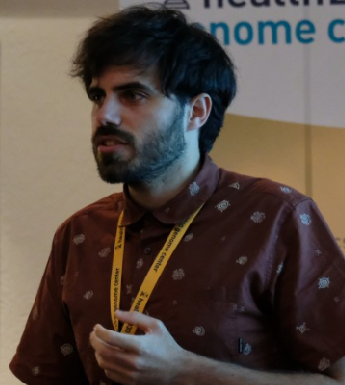
\includegraphics[width=.55\textwidth]{profile}
\end{minipage}


% Subheader
\begin{minipage}[c]{0.65\textwidth}
  \begin{center}
    \href{mailto:david.mas.p@gmail.com}{david.mas.p@gmail.com}\\
    Barcelona, Spain
  \end{center}
\end{minipage}
\begin{minipage}[c]{0.3\textwidth}
\href{https://github.com/davidmasp}{github://davidmasp}

\includegraphics[height=12pt]{gh}\\
\href{https://www.linkedin.com/in/davidmasponte/}{linkedin://davidmasponte}

\includegraphics[height=12pt]{in}\\
\href{http://david.masponte.com/}{david.masponte.com}
\end{minipage}


\vspace{0.75cm}
\rule{.95\textwidth}{0.6pt}

%%%% EDUCATION %%%%

\section*{Education}
\begin{tabular}{L!{\VRule}R}
  2015--2017&{\bf M.Sc. in Bioinformatics for Health Sciences}\\
   & Universitat Pompeu Fabra, Barcelona, Spain.\\
   & {\em \color{black!50} Specialization in Genomics - GPA: 9 / 10 }\\[15pt]
  2014&Exchange Student \\
   &  McGill University, Montreal, Canada.\\
   & {\em \color{black!50} Academic international exchange}\\[15pt]
  2011--2015&B.Sc. in Biotechnology\\
   & Universitat Autonoma de Barcelona, Spain.\\
   & { \em \color{black!50} GPA: 8.5 / 10}
\end{tabular}

%%%% Research %%%%
\section*{Research Experience}
\begin{tabular}{L!{\VRule}R}
08 2017 -  &{\bf Institute for Research in Biomedicine } - {\em \color{black!70} Ph.D. Student }   \\
 & My Ph.D. project is enclosed in the field of computational genetics, studying how mutational processes shape the eukaryotic genomes. We use statistical and machine learning techniques to extract patterns from massive genomic data sets. In particular, we are interested in unraveling mechanisms of local hypermutation both somatically and in populations. {\bf Fran Supek's Lab (AGENDAS)}.\\[15pt]
2016 - 2017&{\bf Centre for Genomic Regulation (CRG) } - {\em \color{black!70} Master Science Research Thesis  }\\
 & My Master Thesis was focused in the link between lncRNAs' subcellular localization and their function. I have also developed a web-based DB using R and SQL to make subcellular expression data available to the scientific community. {\bf Roderic Guigo's Lab, tutored by Rory Johnson}.\\[15pt]
2015-2016 & {\bf Institute of Evolutionary Biology (IBE) } - {\em \color{black!70} Part time Research Internship}\\
 & I studied the evolutionary processes surrounding the RHD gene in Western Mediterranean populations in order to unravel demographic ({\em drift}) or adaptive ({\em selection}) processes. {\bf David Comas' Lab}\\[15pt]
06-08 2014 & {\bf Molecular Biology Institute of Barcelona (IBMB) }- {\em \color{black!70} Research Internship}\\
 &  I took part in the study of the CIC (CapICua) protein in Drosophila development. I gained research skills in fruit fly genetics, in \textit{in situ} hybridization and in recombinant DNA techniques for CRISPR/Cas9 set up. {\bf Gerardo Jimenez's Lab}\\[15pt]
\end{tabular}

\vspace{10pt}

%%%% Programing %%%%

\begin{minipage}{.5\linewidth}
\section*{Code}
\begin{tabular}{L!{\VRule}R}
\tikz\draw[black,fill=black] (0,0) circle (.7ex); 
\tikz\draw[black,fill=black] (0,0) circle (.7ex);
\tikz\draw[black,fill=black] (0,0) circle (.7ex); & R, Python, Bash \& nextflow  \\
\tikz\draw[black,fill=black] (0,0) circle (.7ex); 
\tikz\draw[black,fill=black] (0,0) circle (.7ex);
\tikz\draw[black] (0,0) circle (.7ex); & Docker, git  \&  \LaTeX \\
\tikz\draw[black,fill=black] (0,0) circle (.7ex); 
\tikz\draw[black] (0,0) circle (.7ex);
\tikz\draw[black] (0,0) circle (.7ex); & SQL, JavaScript \& HTML/CSS
\end{tabular}
\end{minipage}
\begin{minipage}{.5\linewidth}
%%%% lang %%%%
\section*{Languages}
\begin{tabular}{L!{\VRule}R}
Catalan & Mother tongue\\
Spanish & Bilingual Proficiency\\
{\bf English}&{\bf Proficient (CAE-C2 2021)}
\end{tabular}
\end{minipage}


%%%% pubs %%%%

\bibliographystyle{unsrtnat}
\nobibliography{dmas}

\section*{Selected Publications} 

Find a complete list at \href{https://orcid.org/0000-0001-7409-305X}{orcid.org/0000-0001-7409-305X}.
\\
\\
\begin{tabular}{L!{\VRule}R}
2020 & \bibentry{mas_dna_2020} - {\em \color{black!70} Peer-reviewed Journal}\\
 &  \bibentry{carlevaro-fita_cancer_2020} - {\em \color{black!70} Peer-reviewed Journal}\\[60pt]
 2019 &  \textbf{} \bibentry{salvadores_passenger_2019}- {\em \color{black!70} Peer-reviewed Journal} \\
& \bibentry{franco_whole_2019} - {\em \color{black!70} Peer-reviewed Journal} \\[60pt]
2017 & \bibentry{mas-ponte_lncatlas_2017} - {\em \color{black!70} Peer-reviewed Journal}\\[5pt]
\end{tabular}


\section*{Selected Conferences}



\begin{tabular}{L!{\VRule}R}
2021 &\textbf{}\bibentry{mas_EACR_2021} - {\em \color{black!70} Peer-reviewed Conference - Short talk} \\[30pt]
2019 &\textbf{}\bibentry{david_mas-ponte_hypermut_2019} - {\em \color{black!70} Peer-reviewed Conference - Poster} \\[30pt]
2018 &\textbf{}\bibentry{david_mas-ponte_association_2018} - {\em \color{black!70} Peer-reviewed Conference - Poster} \\
\end{tabular}

%%%% SA %%%%
\section*{Other scientific contributions \& Awards}

\begin{tabular}{L!{\VRule}R}
2021 & \textbf{SCB award to the best scientific article} -  {\em \color{black!70} Nominee}   \\
& The \textit{Societat Catalana de Biologia} (SCB) is the society that groups all professional and academic biologist
in Catalonia. Every year, they award a recognition to the best scientific article in life sciences published in an international journal. In 2021, my paper (\textit{Mas-Ponte Nature Genetics 2020}) got selected as one of the nominees for this award \\[60pt]
2018-2019 & \textbf{ENABLE 2019} -  {\em \color{black!70} Scientific Organizing Committee}   \\
& ENABLE is an international scientific conference for Ph.D. Students from all over the world co-organized by 4 European research centers (IRB Barcelona, RIMLS, CPR, and SEMM) funded by the European Union Horizon 2020 program. The third edition was held in the city of Nijmegen in the Netherlands with a total of 229 Ph.D. students and postdocs coming from 26 different countries.
 \end{tabular}





\end{document}
